\documentclass{article}

\usepackage[T2A]{fontenc}
\usepackage[utf8]{luainputenc}
\usepackage[english, russian]{babel}
\usepackage[pdftex]{hyperref}
\usepackage[14pt]{extsizes}
\usepackage{listings}
\usepackage{color}
\usepackage{geometry}
\usepackage{subcaption}
\usepackage{enumitem}
\usepackage{multirow}
\usepackage{graphicx}
\usepackage{indentfirst}
\usepackage[ruled,vlined,linesnumbered]{algorithm2e}

\setlength{\parskip}{3mm}
\geometry{a4paper,top=20mm,bottom=20mm,left=25mm,right=15mm}
\setlist{nolistsep, itemsep=0.5cm,parsep=0pt}

\lstset{
  backgroundcolor=\color{gray!10},
  basicstyle=\fontsize{13}{13}\ttfamily,
  columns=fullflexible,
  breakatwhitespace=false,
  breaklines=true,
  captionpos=b,
  extendedchars=true,
  frame=single,
  keepspaces=true,
  keywordstyle=\color{blue},
  language=c++,
  numbers=none,
  numbersep=1pt,
  numberstyle=\tiny\color{blue},
  rulecolor=\color{mygray},
  showspaces=false,
  showtabs=false,
  stringstyle=\color{mymauve},
  title=\lstname
}

\makeatletter
\renewcommand\@biblabel[1]{#1.\hfil}
\makeatother

\begin{document}

\begin{titlepage}

\begin{center}
Министерство науки и высшего образования Российской Федерации \\
\vspace{5mm}
Федеральное государственное автономное образовательное учреждение высшего образования \\
Национальный исследовательский Нижегородский государственный университет им. Н.И. Лобачевского \\
\vspace{1cm}
Институт информационных технологий, математики и механики \\
\vspace{5cm}
\textbf{\large Отчет по лабораторной работе} \\
\vspace{8mm}
\textbf{\Large «Поразрядная сортировка для вещественных чисел (тип double) с четно-нечетным слиянием Бэтчера»} \\
\end{center}

\vspace{3cm}

\newbox{\lbox}
\savebox{\lbox}{\hbox{text}}
\newlength{\maxl}
\setlength{\maxl}{\wd\lbox}
\hfill\parbox{7cm}{
\hspace*{5cm}\hspace*{-5cm}\textbf{Выполнил:} \\ студент группы 381706-1 \\ Суслов Е. И.\\
\\
\hspace*{5cm}\hspace*{-5cm}\textbf{Проверил:} \\ доцент кафедры МОСТ, \\ кандидат технических наук \\ Сысоев А. В.
}

\vspace{\fill}

\begin{center}
Нижний Новгород \\ 2020
\end{center}
\end{titlepage}

\setcounter{page}{2}

\tableofcontents

\newpage

\section{Введение}

\par Алгоритмом сортировки называется алгоритм для упорядочения некоторого множества элементов. Обычно под алгоритмом сортировки подразумевают алгоритм упорядочивания множества элементов по возрастанию или убыванию.

В случае наличия элементов с одинаковыми значениями, в упорядоченной последовательности они располагаются рядом друг за другом в любом порядке. Однако иногда бывает полезно сохранять первоначальный порядок элементов с одинаковыми значениями.

В алгоритмах сортировки лишь часть данных используется в качестве ключа сортировки. Ключом сортировки называется атрибут (или несколько атрибутов), по значению которого определяется порядок элементов. Таким образом, при написании алгоритмов сортировок массивов следует учесть, что ключ полностью или частично совпадает с данными.

Практически каждый алгоритм сортировки можно разбить на 3 части:
\begin{itemize}
\item сравнение, определяющее упорядоченность пары элементов;

\item перестановку, меняющую местами пару элементов;
\item собственно сортирующий алгоритм, который осуществляет сравнение и перестановку элементов до тех пор, пока все элементы множества не будут упорядочены.
\end{itemize}
Алгоритмы сортировки имеют большое практическое применение. Их можно встретить там, где речь идет об обработке и хранении больших объемов информации. Некоторые задачи обработки данных решаются проще, если данные заранее упорядочить.

\par Ни одна другая проблема не породила такого количества разнообразнейших решений, как задача сортировки. Универсального, наилучшего алгоритма сортировки на данный момент не существует. Однако, имея приблизительные характеристики входных данных, можно подобрать метод, работающий оптимальным образом. Для этого необходимо знать параметры, по которым будет производиться оценка алгоритмов.
\begin{itemize}
\item Время сортировки – основной параметр, характеризующий быстродействие алгоритма.
\item Память – один из параметров, который характеризуется тем, что ряд алгоритмов сортировки требуют выделения дополнительной памяти под временное хранение данных. При оценке используемой памяти не будет учитываться место, которое занимает исходный массив данных и независящие от входной последовательности затраты, например, на хранение кода программы.
\item Устойчивость – это параметр, который отвечает за то, что сортировка не меняет взаимного расположения равных элементов.
\item Естественность поведения – параметр, которой указывает на эффективность метода при обработке уже отсортированных, или частично отсортированных данных. Алгоритм ведет себя естественно, если учитывает эту характеристику входной последовательности и работает лучше.
\end{itemize}
Классификация алгоритмов сортировок
Все разнообразие и многообразие алгоритмов сортировок можно классифицировать по различным признакам, например, по устойчивости, по поведению, по использованию операций сравнения, по потребности в дополнительной памяти, по потребности в знаниях о структуре данных, выходящих за рамки операции сравнения, и другие.

Наиболее подробно рассмотрим классификацию алгоритмов сортировки по сфере применения. В данном случае основные типы упорядочивания делятся следующим образом.
\begin{itemize}
\item Внутренняя сортировка – это алгоритм сортировки, который в процессе упорядочивания данных использует только оперативную память (ОЗУ) компьютера. То есть оперативной памяти достаточно для помещения в нее сортируемого массива данных с произвольным доступом к любой ячейке и собственно для выполнения алгоритма. Внутренняя сортировка применяется во всех случаях, за исключением однопроходного считывания данных и однопроходной записи отсортированных данных. В зависимости от конкретного алгоритма и его реализации данные могут сортироваться в той же области памяти, либо использовать дополнительную оперативную память.
\item Внешняя сортировка – это алгоритм сортировки, который при проведении упорядочивания данных использует внешнюю память, как правило, жесткие диски. Внешняя сортировка разработана для обработки больших списков данных, которые не помещаются в оперативную память. Обращение к различным носителям накладывает некоторые дополнительные ограничения на данный алгоритм: доступ к носителю осуществляется последовательным образом, то есть в каждый момент времени можно считать или записать только элемент, следующий за текущим; объем данных не позволяет им разместиться в ОЗУ.
\end{itemize}
Внутренняя сортировка является базовой для любого алгоритма внешней сортировки – отдельные части массива данных сортируются в оперативной памяти и с помощью специального алгоритма сцепляются в один массив, упорядоченный по ключу.

Следует отметить, что внутренняя сортировка значительно эффективней внешней, так как на обращение к оперативной памяти затрачивается намного меньше времени, чем к носителям.

\par Многообразие сортировок это хорошо, но даже у самой хорошо подобранной под задачу сортировки существует свой предел производительности, чтобы решить эту проблему можно использовать возможности паралелизма на современных многопроцессных и многопоточных процессорах.

\par Для использования многопоточности существуют несколько технологий самыми популярными из которых являются следующие: Intel Threading Building Blocs, Open Multi-Processing или std::thread.
Для каждой из этих технологий существует свой синтаксис; свои плюсы, минусы и ограничения.

\par В данной работе будут представлены возможности по распараллеливаню последовательной реализации поразрядной сортировки для вещественных чисел (тип double) с четно-нечетным слиянием Бэтчера и произведено сравнение времени их выполнения на всех трех технологиях многопоточности представленных выше.

\newpage

\section{Постановка задачи}
Формулировка задачи:

\begin{enumerate}
\item Реализовать последовательный алгоритм поразрядной сортировки для вещественных чисел (тип double) с четно-нечетным слиянием Бэтчера.
\item Ускорить работу алгоритма используя технологии многопоточности(OpenMP, TBB и std::threads).
\item Реализовать набор автоматических тестов с использованием Google C++ Testing Framework для последовательной и параллельных реализаций алгоритма.
\item Сравнить ускорения достигнутые на каждой из технологий по сравнению с последовательной реализацией.
\end{enumerate}

\newpage

\section{Метод решения}
\subsection{Поразрядная сортировка}

\par Поразрядная сортировка имеет две модификации: Most Significant Digit (MSD) и Least Significant Digit (LSD).
\par В данной работе будет рассмотрен алгоритм LSD как наиболее эффективный. Идея поразрядной восходящей сортировки (Least Significant Digit (LSD) Radix Sort) заключается в том, что выполняется последовательная сортировка чисел по разрядам (от младшего разряда к старшему).
\par Поразрядная сортировка массива будет работать только в том случае, если сортировка, выполняющаяся по разряду, является устойчивой (элементы равных разрядов не будут менять взаимного расположения при сортировке по очередному разряду).
\par Современные процессоры предназначены для обработки данных, которые представлены в битах и байтах, поэтому выполнять сортировку по десятичным разрядам чисел не эффективно. Рассмотрим побайтовую реализацию поразрядной сортировки, т.е. будем рассматривать число как набор 256-значных цифр. В таком случае для сортировки разряда будет удобно использовать сортировку подсчѐтом (с модификацией, которая не будет менять взаимного расположения элементов равных разрядов).
\par Сортировка подсчѐтом по i-му байту будет проходить в два прохода по исходному массиву:
\begin{itemize}
\item при первом проходе по исходному массиву выполняется подсчѐт i-ых байт в массиве mas, результат будет сохранѐн в массив подсчѐтов counter из 256 элементов;
\item в массив offset на основании посчитанных данных выполняется подсчѐт смещений, по которым будут сохраняться элементы: \\
offset[0] = 0 \\
для всех j от 1 до 255  \\
offset[j] = counter[j-1] + offset[j-1]
\item при втором проходе по исходному массиву mas выполняется копирование элемента во вспомогательный массив по соответствующему индексу в массиве смещений offset и выполняется инкремент смещения.
\end{itemize}
\par Принятие стандарта IEEE 754 в 1985 году ознаменовало новую эру в области вычислительной математики. Появились единые стандарты на реализацию элементарных операций, математических функций, представление данных разной точности в памяти ЭВМ, правила округления и т.д. Подробное рассмотрение стандарта выходит за рамки данной работы, ограничимся лишь некоторой описательной информацией по поводу представления чисел с плавающей запятой двойной точности, необходимой для понимания алгоритмов сортировки.
\par Рассмотрим кратко, как представляются числа типов float (одинарная точность) и double (двойная точность) в памяти ЭВМ. В соответствии со стандартом IEEE 754 для хранения числа отводится три поля: знак, смещенный порядок и мантисса.


\begin{center}
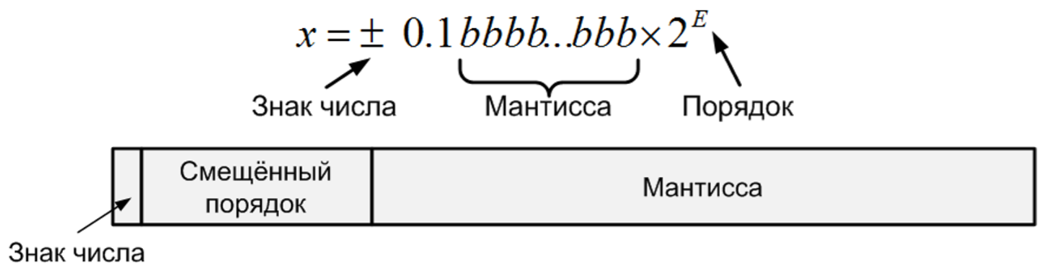
\includegraphics[width=1\textwidth]{../../../../modules/reports/suslov_e_radix_with_batchers_merge/IEEE.png}
\captionof{figure}{Хранение вещественных чисел по стандарту IEEE 754}\label{visina1}
\end{center}

Старший бит типов с плавающей точкой кодирует знак числа, поэтому сортировка по старшему биту должна выполняться в обратном порядке (1 “меньше” 0). Для положительных чисел большее значение порядка соответствует большему числу, т.к:
\begin{itemize}
\item в случае нормализованного представления неявный старший бит мантиссы равен 1;
\item в случае денормализованного представления значение поля соответствует минимальному, а неявный старший бит мантиссы равен 0.
\end{itemize}
\par Для положительных чисел в случае равенства порядка, большее значение мантиссы соответствует большему числу. Таким образом, побайтовая сортировка положительных чисел допустима и по всем байтам должна выполняться в обычном порядке (0 “меньше” 1).
\par Для отрицательных чисел большее значение порядка соответствует меньшему числу (рассуждения аналогичны рассуждениям о положительных числах). Таким образом, сортировка отрицательных чисел по всем байтам должна выполняться в обратном порядке (1 “меньше” 0).
Общий алгоритм сортировки типов с плавающей точкой:
\begin{itemize}
\item сортировка чисел по старшему биту, разделяя числа на две группы: отрицательные и положительные;
\item для положительных чисел сортировка по всем байтам выполняется в обычном порядке (0 “меньше” 1);
\item для отрицательных чисел сортировка по всем байтам выполняется в обратном порядке (1 “меньше” 0).
\end{itemize}
\subsection{Четно-нечетное слияние Бэтчера}
\par Четно-нечетное слияние Бэтчера заключается в том, что два упорядоченных массива, которые необходимо слить, разделяются на чѐтные и нечѐтные элементы. Далее выполняется слияние четных и нечетных элементов массивов. Такое слияние может быть выполнено параллельно.
\par Чтобы массив стал окончательно отсортированным, достаточно сравнить пары элементов, стоящие на нечетной и чѐтной позициях. Первый и последний элементы массива проверять не надо, т.к. они являются минимальным и максимальным элементов массивов.
\par Четно-нечетное слияние Бэтчера позволяет задействовать 2 потока при слиянии двух упорядоченных массивов. В этом случае слияние n массивов могут выполнять n параллельных потоков. На следующем шаге слияние n/2 полученных массивов будут выполнять n/2 потоков и т.д. На последнем шаге два массива будут сливать 2 потока.
\begin{center}
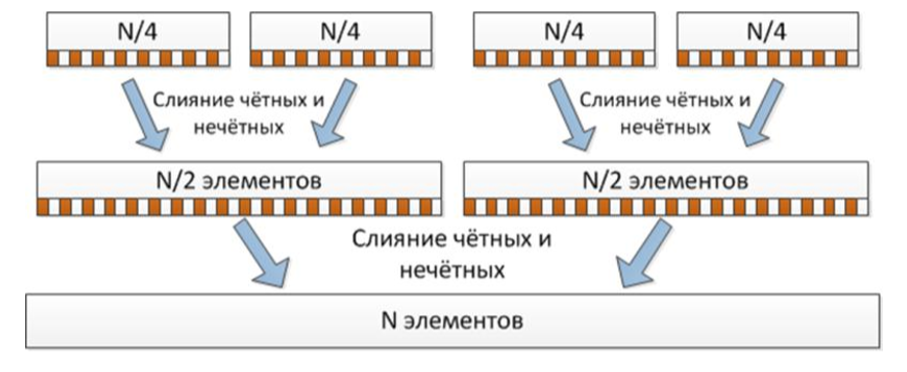
\includegraphics[width=1\textwidth]{../../../../modules/reports/suslov_e_radix_with_batchers_merge/Batcher_merge.png}
\captionof{figure}{Четно-нечетное слияние Бэтчера}\label{visina1}
\end{center}
\newpage

\section{Схема распараллеливания}
Последовательный алгоритм представляет собой рекурсивное деление всего массива на два подмассива (до определенного размера, после достижения которого части массива отправляются в функцию реализующую побайтовую восходящую сортировку), которые, после сортировки каждого поразрядой сортировки, сливаются четно-нечетным слиянием Бэтчера:
\vspace{10pt}
\begin{lstlisting}
    void LSDParallelSorter(double* mas, double* tmp, int size, int portion) {
    if (size <= portion) {
        LSDSortDouble(mas, tmp, size);
    } else {
        int elem = size / 2 + (size / 2) % 2;
        LSDParallelSorter(mas, tmp, elem, portion);
        LSDParallelSorter(mas + elem, tmp + elem, size - elem, portion);
        EvenSplitter(mas, tmp, elem, size - elem);
        OddSplitter(mas, tmp, elem, size - elem);
        SimpleComparator(mas, size);
    }
}
\end{lstlisting}
\vspace{-25pt}

\par При таком делении массива, разделенные части остаются независимыми друг от друга до их полной сортировки и возврата управления в вызвавшую их функцию (расположенную на на уровень выше в дереве рекурсии), после полной сортировки подмассивов возможно выполнить четно-нечетное слияние Бэтчера. Преимущество этого слияния в том что оно может быть выполнено в два потока (одновременно для четных и для нечетных элементвов массивов).
Также необходимо учитывать, что одна из двух функций рекурсии может выполнится быстрее соседней, в таком случае необходимо синхронизировать их завершение до вызова функций слияния, иначе будем сливать неосортированный массив и отсортированный.

\par Наиболее эффективными параллельными алгоритмами являются те, которые имеют внутренний параллелизм, поэтому рассмотрим параллельный алгоритм побайтовой сортировки.

\par Алгоритм побайтовой сортировки заключается в последовательном применении сортировки подсчѐтом к каждому байту чисел, поэтому параллельно может выполняться только сортировка подсчѐтом для каждого байта. Сортировка подсчѐтом состоит из двух этапов: подсчѐт количества элементов и их размещение. Первый этап может быть выполнен параллельно над частями массива и в последующем редуцирован. Второй этап может быть выполнен параллельно только в том случае, если при его выполнении будет сохраняться свойство устойчивости сортировки. Для этого достаточно пересчитать смещения для каждой порции массива. Приведем лишь его словесное описание, так как для нашего тестового массива в 100 млн он не дает преимущества во времени.

\par Параллельный алгоритм сортировки подсчѐтом будет состоять из следующих шагов:

\begin{enumerate}
\item Для каждого потока создаѐтся массив подсчѐтов и заполняется нулями. \item Каждый поток получает на обработку часть массива и выполняет подсчѐт элементов в свой массив подсчѐтов.
\item С помощью массивов подсчѐтов со всех потоков выполняется вычисление смещений, по которым будут располагаться элементы при втором проходе по массиву.
\itemКаждый поток получает на обработку ту же часть массива, что и ранее, и выполняет копирование элемента во вспомогательный массив по соответствующему индексу в массиве смещений.
\end{enumerate}
\par Такой алгоритм имеет смысл для больших данных, иначе, как и в нашем случае, накладные расходы замедляют работу настолько, что последовательная версия выполняется не медленнее параллельной.

\par Далее будут рассмотрены практические реализации всех возможностей параллелизма на этой задаче, т.е. будут применены технологии OpenMP, TBB и std::threads, с целью уменьшить скорость выполнения нашего алгоритма.

\subsection{OpenMP}
Для использования OpenMP необходимо подключить \verb|<omp.h>|.
\par Перед выполнением кода в представленной ниже листинге необходимо включить вложенный параллелизм:
\vspace{10pt}
\begin{lstlisting}
omp_set_nested(1);
\end{lstlisting}
\vspace{-25pt}
\par Рассмотрим основные моменты синтаксиса используемые в представленной реализации.\\
Создаем два потока:
\vspace{10pt}
\begin{lstlisting}
#pragma omp parallel num_threads(2)
\end{lstlisting}
\vspace{-25pt}
Допускаем один поток к выполнению задачу и сообщаем что ожидать его выполнения не нужно:
\vspace{10pt}
\begin{lstlisting}
#pragma omp single nowait
\end{lstlisting}
\vspace{-25pt}
Ожидаем полной сортировки двух подмассивов до вызова функций четно-нечетного слияния Бэтчера:
\vspace{10pt}
\begin{lstlisting}
#pragma omp barrier
\end{lstlisting}
\vspace{-25pt}

В итоге получим:
\vspace{10pt}
\begin{lstlisting}
   #pragma omp parallel num_threads(2)
                {
#pragma omp single nowait
                    {
                        LSDParallelSorterOMP(mas, tmp, elem, portion, lvl);

                    }
#pragma omp single nowait
                    {
                        LSDParallelSorterOMP(mas + elem, tmp + elem, size - elem, portion, lvl);
                    }
#pragma omp barrier
#pragma omp single nowait
                    {
                        EvenSplitter(mas, tmp, elem, size - elem);
                    }
#pragma omp single nowait
                    {
                        OddSplitter(mas, tmp, elem, size - elem);
                    }
#pragma omp barrier
#pragma omp single nowait
                    {
                        SimpleComparator(mas, size);
                    }
                }
\end{lstlisting}
\vspace{-25pt}

Также можно распараллелить по потокам проход по массиву после сливания четных и нечетных элементов, он необходим, т.к. соседние элементы могут стоять не в правильном порядке (первый и последний элементы проверять не нужно). Его удобнее реализовать с помощью встроенного синтаксиса распределения нагрузки при исполнении итераций цикла по потокам (будет создано удобное для нашего "железа" количество потоков или заранее заданное).
\vspace{10pt}
\begin{lstlisting}
    #pragma omp parallel for
for (int i = 1; i < (size+1)/2; i++)
    if (mas[2 * i] < mas[2 * i - 1]) {
        double _tmp = mas[2 * i - 1];
        mas[2 * i - 1] = mas[2 * i];
        mas[2 * i] = _tmp;
    }
}
\end{lstlisting}
\vspace{-25pt}

\subsection{TBB}
Для использования TBB необходимо подключить \verb|<tbb/tbb.h>|.
TBB представляет более широкие возможности для реализации многопоточных алгоритмов, поэтому будет целесообразно обернуть функции из последовательного алгоритма в классы, с которыми TBB приобретает наибольшую функциональность.
\vspace{10pt}
\begin{lstlisting}
class EvenSplitter;
class OddSplitter;
class SimpleComparator;
class LSDParallelSorter;
\end{lstlisting}
\vspace{-25pt}
\par Синтаксис последнего класса выглядит так:
\vspace{10pt}
\begin{lstlisting}
    class LSDParallelSorter :public tbb::task {
 private:
    double* mas;
    double* tmp;
    int size;
    int portion;

 public:
    LSDParallelSorter(double* _mas, double* _tmp, int _size, int _portion) :
        mas(_mas), tmp(_tmp), size(_size), portion(_portion)
    {}
    task* execute() {
        if (size <= portion) {
            LSDSortDouble(mas, tmp, size);
        } else {
            int s = size / 2 + (size / 2) % 2;
            LSDParallelSorter& sorter1 = *new (allocate_child())
                LSDParallelSorter(mas, tmp, s, portion);
            LSDParallelSorter& sorter2 = *new (allocate_child())
                LSDParallelSorter(mas + s, tmp + s, size - s,
                    portion);
            set_ref_count(3);
            spawn(sorter1);
            spawn_and_wait_for_all(sorter2);
            EvenSplitter& splitter1 = *new (allocate_child())
                EvenSplitter(mas, tmp, s, size - s);
            OddSplitter& splitter2 = *new (allocate_child())
                OddSplitter(mas, tmp, s, size - s);
            set_ref_count(3);
            spawn(splitter1);
            spawn_and_wait_for_all(splitter2);
            tbb::parallel_for(tbb::blocked_range<int>(1, (size + 1) / 2),
                SimpleComparator(mas, size));
        }
        return NULL;
    }
};
\end{lstlisting}
\vspace{-25pt}
Параллелизма в TBB в данной реализации достигается за счет добавления задач в пулл задач и затем их исполнением свободными потоками. Как видно из листинга:
\begin{enumerate}
\item Cначала добавляются задачи осуществляющие рекурсию (т.е.деление массива до необходимой длины установленной в portion): sorter1, sorter2.

\item Заставляем ожидать исполнения всех задач которые являются потомками текущих двух.
\item Аналогично создаем задачи на четное и нечетное сливание сооветственно и дожидаемся их исполнения.
\item Встроенным синтаксисом TBB создаем одномерное итерационное пространство по которому будет итерироваться распределитель цикла по потокам и раздавать задания потокам.
\end{enumerate}

\subsection{std::threads}

\par Для использования возможностей \verb|std::threads| необходимо подключить \verb|<thread>|. Так как нам особый функционал для управления потоками не нужен, то можно предоставить это самой технологии \verb|std::threads| и создавать асинхронные потоки  \verb|std::async|. Так они возвращают объект типа \verb|future|, то необходимо подключить соответствующую библиотеку \verb|<future>|.

\par Все остальное аналогично за исключением того, что добиваемся правильного порядка с помощью следующего синтаксиса \verb|t1.wait()| (в примере к ожиданию t1 ~--- первого объекта \verb|future| ):
\vspace{10pt}
\begin{lstlisting}
void LSDParallelSorter(double* mas, double* tmp, int size, int portion) {
    if (size <= portion) {
        auto t0 = std::async(LSDSortDouble, mas, tmp, size);
    } else {
        int elem = size / 2 + (size / 2) % 2;
        auto t1 = std::async(LSDParallelSorter, mas, tmp, elem, portion);
        auto t2 = std::async(LSDParallelSorter, mas + elem, tmp + elem, size - elem, portion);
        t1.wait();
        t2.wait();
        auto t3 = std::async(EvenSplitter, mas, tmp, elem, size - elem);
        auto t4 = std::async(OddSplitter, mas, tmp, elem, size - elem);
        t3.wait();
        t4.wait();
        auto t5 = std::async(SimpleComparator, mas, size);
    }
}
\end{lstlisting}
\vspace{-25pt}

\newpage

\section{Подтверждение корректности}
Для проверки корректности выполнения программы для каждой из технологий был реализован набор тестов, разработанных с помощью Google C++ Testing Framework.

Для удобства создания тестов созданы функции:\\
Для копирования массива
\vspace{10pt}
\begin{lstlisting}
double* array_double_copy(double* Array, int size)
\end{lstlisting}
\vspace{-25pt}
Для проверки идентичности массивов
\vspace{10pt}
\begin{lstlisting}
bool CompareArrays(double* mas, double* Mas, int size)
\end{lstlisting}
\vspace{-25pt}

Структура тестов представляет собой создание double массива определенной длины, его копирование с помощью функции, затем сортировки исходного массива написанным алгоритмом, а массива копии алгоритмом реализованным в стандартной библиотеке \verb|std::sort| или \verb|tbb::parallel_sort|. Затем оба массива загоняются в функцию поэлементной сверки идентичности массивов, которая возвращает 1 если массивы одинаковы и 0 в обратном случае.

\par Далее с помощью функционала тестов осуществляется проверку вывод функции проверки идентичности массивов с 1.
\vspace{10pt}
\begin{lstlisting}
ASSERT_EQ(1, CompareArrays(Array, Array_copy, size));
\end{lstlisting}
\vspace{-25pt}

\par Таким образом осуществляется проверка каждой реализации алгоритма (как минимум 5-ю тестами).

Так как все тесты выполняются успешно, то можно гарантировать корректность реализованного алгоритма сортировки массива случайных чисел типа \verb|double|.
\newpage

\section{Результаты экспериментов}
Вычислительные эксперименты для оценки эффективности параллельного варианта поразрядной сортировки с четно-нечетным слиянием Бэтчера проводились на ноутбуке со следующими характеристиками:

\begin{itemize}
\item ОС: Microsoft Windows 10 Pro;
\item CPU: AMD Ryzen 5 3500U with Radeon Vega Mobile Gfx (2,10ГГц);
\item Число ядер: 4;
\item Логических процессоров: 8;
\item Оперативная память: 8 Гб из которых доступно 2.9 Гб (2400 MГц);
\item Размер кэшов L1, L2, L3: 384 Кб, 2.0 Мб, 4.0 Мб соответственно;
\end{itemize}

\par Замер времени производился при сортировке массива в 100 млн \verb|double| чисел, количество потоков для выполнения выбиралось оптимальное для конкретной технологии и реализации, так в OpenMP использовалось 8 потоков, в TBB 4 потока, а в std::thread количество потоков подбиралось автоматически. Время усреднялось по результату 8 замеров, следующих друг за другом.

\begin{tabular}{ | l | l | }
\hline
\textbf{Технология} & \textbf{Время в секундах}  \\ \hline
Последовательно & 12,3655  \\
OpenMP & 4,470125  \\
TBB & 3,6885   \\
std::thread & 3,9185 \\
\hline
\end{tabular}
\par По итогу, по сравнению с последовательной реализацией алгоритма, OpenMP дает усредненное ускорение (на оптимальном количпстве потоков) в 2.766, ТВВ в 3.352, std::thread в 3,155 раза.

\begin{center}
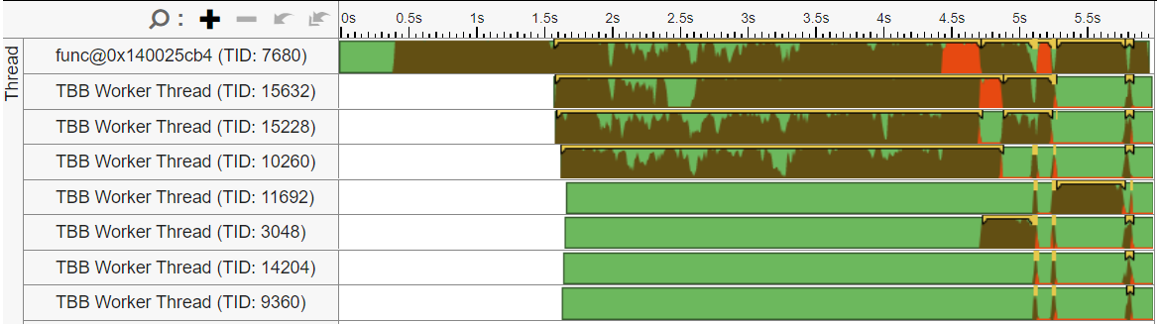
\includegraphics[width=1\textwidth]{../../../../modules/reports/suslov_e_radix_with_batchers_merge/TBB.png}
\captionof{figure}{Распределение нагрузки между потоками в TBB}\label{visina1}
\end{center}

\begin{center}
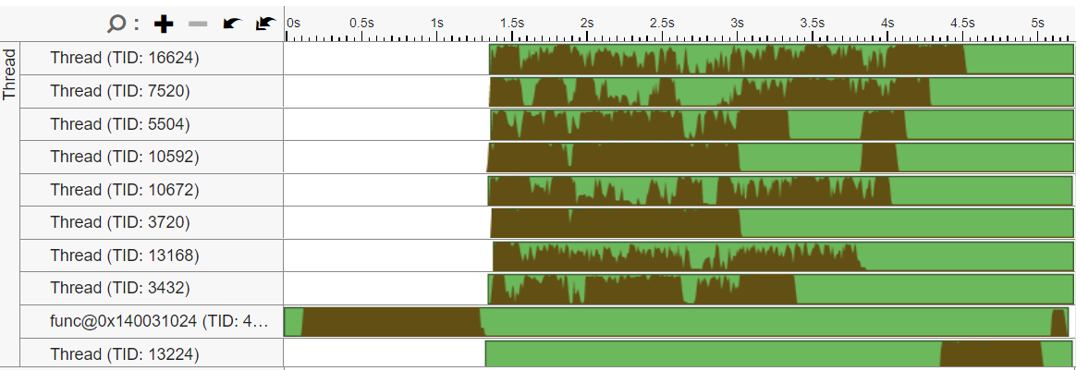
\includegraphics[width=1\textwidth]{../../../../modules/reports/suslov_e_radix_with_batchers_merge/thread_.png}
\captionof{figure}{Распределение нагрузки между потоками в std::threads}\label{visina1}
\end{center}

\par По наглядному представлению загрузки потоков видно, что std::threads тратит много времени на распределение нагрузки между большим количеством потоков, из-за чего тратит много времени, а TBB обратно загружает практически польностью первые четыре потока, благодаря чему видимо и экономит немного времени.
\par OpenMP же, в моей реализации, загружает работой два потока полностью, а остальные подключаются при сравнении соседних элементов, о чем и свидетельствует полученное ускорение.
\newpage

\section{Заключение}
По итогу все поставленные задачи выполнены.

\par В ходе выполнения данной работы были изучены алгоритмы: поразрядной сортировки для вещественных чисел (тип double) и  четно-нечетного слияния Бэтчера. Данные алгоритмы были реализованы на языке высокого уровня С++.

\par Успешно выполнена и протестирована многопоточная (параллельная) реализация с использованием технологий: OpenMP, TBB, std::threads.

\par Разработаны и успешного выполнены тесты, созданные с использованием Google C++ Testing Framework.

\par Были проведены эксперименты, по результатам лучшей технологией для реализации параллельного алгоритма поразрядной сортировки для вещественных чисел (тип double) и  четно-нечетного слияния Бэтчера оказалась библиотека TBB, но остальные реализации не сильно отстали по времени выполнения. То что порог вхождения для написания программы на OpenMP и std::threads гораздо ниже чем на TBB также играет не в пользу последней.
\par Подытоживая можно сказать что TBB представляет наиболее широкий функционал, в OpenMP наиболее просто можно распараллелить базовые конструкции, преимущество std::threads в том что не требуется дополнительная установка на пк средств распараллеливания, а также гибкость в принятии модели параллелизма (std::thread, std::async).
\par В целом можно сказать что каждая из технологий имеет право на существование. Но наибольшее удовольствие представляет распараллеливание цикла for в OpenMP и использование асинхронных потоков в std::threads.

\newpage

\section{Список литературы}
\begin{enumerate}

\bibitem{TBB} А.А. Сиднев, А.В. Сысоев, И.Б. Мееров. Образовательный комплекс  «Параллельные численные методы» , Лабораторная работа №3 Сортировки. Нижний Новгород, ННГУ, 2010, 65 с.

\bibitem{OMP} Гергель В.П. Учебный курс «Введение в методы параллельного программирования», раздел «Параллельное программирование с использованием OpenMP». Нижний Новгород, ННГУ, 2007, 33 с.

\bibitem{TBB} А.А. Сиднев, А.В. Сысоев, И.Б. Мееров. Учебный курс «Технологии разработки параллельных программ», раздел «Создание параллельной программы», «Библиотека Intel Threading Building Blocks~--- краткое описание». Нижний Новгород, ННГУ, 2007, 29 с.

\bibitem{STD} Справочник по конструкциям языка C++, раздел std::thread // URL: https://ru.cppreference.com/

\bibitem{TBB} Введение в параллельные методы решения задач: Учебное пособие / Предисл.: В. А. Садовничий. – М.: Издательство Московского университета, 2013. – 328 с., илл. – (Серия «Суперкомпьютерное образование»)
\end{enumerate}

\newpage

\section{Приложение}
\subsection{Последовательный алгоритм поразрядной сортировки для вещественных чисел (тип double) и  четно-нечетного слияния Бэтчера.}
\lstinputlisting[language=C++]{../../../../modules/task_1/suslov_e_sort_batcher/suslov_e_sort_batcher.h}
\lstinputlisting[language=C++]{../../../../modules/task_1/suslov_e_sort_batcher/suslov_e_sort_batcher.cpp}
\lstinputlisting[language=C++]{../../../../modules/task_1/suslov_e_sort_batcher/main.cpp}

\subsection{OpenMP}
\lstinputlisting[language=C++]{../../../../modules/task_2/suslov_e_radix_omp/suslov_e_radix_omp.h}
\lstinputlisting[language=C++]{../../../../modules/task_2/suslov_e_radix_omp/suslov_e_radix_omp.cpp}
\lstinputlisting[language=C++]{../../../../modules/task_2/suslov_e_radix_omp/main.cpp}

\subsection{TBB}
\lstinputlisting[language=C++]{../../../../modules/task_3/suslov_e_radix_b_tbb/suslov_e_radix_b_tbb.h}
\lstinputlisting[language=C++]{../../../../modules/task_3/suslov_e_radix_b_tbb/suslov_e_radix_b_tbb.cpp}
\lstinputlisting[language=C++]{../../../../modules/task_3/suslov_e_radix_b_tbb/main.cpp}

\subsection{std::threads}
\lstinputlisting[language=C++]{../../../../modules/task_4/suslov_e_batchers_sort/suslov_e_batchers_sort.h}
\lstinputlisting[language=C++]{../../../../modules/task_4/suslov_e_batchers_sort/suslov_e_batchers_sort.cpp}
\lstinputlisting[language=C++]{../../../../modules/task_4/suslov_e_batchers_sort/main.cpp}

\end{document}